\documentclass{article}
\usepackage[utf8]{inputenc}
\usepackage{mathtools}
\usepackage{pgfplots}
\usepackage{enumitem}
\usepackage{multicol}
\pgfplotsset{compat=1.13}
\newcommand\tab[1][1cm]{\hspace*{#1}}
\newcommand\limxa{\lim_{x\to a}}
\newcommand\limhz{\lim_{h\to 0}}
\newcommand\limxar{\lim_{x\to a^+}}
\newcommand\limxal{\lim_{x\to a^-}}
\newcommand\limtz{\lim_{\theta\to0}}
\newcommand\ddx{\frac{d}{dx}}
\newcommand\dd[2]{\frac{d{#1}}{d{#2}}}
\newcommand\fx{\(f(x)\) }
\newcommand\ciab{\([a, b]\) }
\newcommand\regsum{\sum_{k=1}^{n}}
\DeclarePairedDelimiter\ceil{\lceil}{\rceil}
\DeclarePairedDelimiter\floor{\lfloor}{\rfloor}

\title{Calculus 1 Notes}
\author{Connor D}
\date{February 2017}

\begin{document}

\maketitle

\subsubsection*{Note: section numbers in this document do not match the section numbers of the course}

\section{Limits}
    The limit is the value that a function approaches as the input approaches some other value. They are denoted
    \begin{gather*}
        \limxa f(x)
    \end{gather*}
    This is the limit of \(f(x)\) as \(x\) approaches \(a\). One sided limits refer to the limit as the input approaches a value from one side. The right sided limit is denoted
    \begin{gather*}
        \limxar f(x)
    \end{gather*}
    While the left sided limit is denoted
    \begin{gather*}
        \limxal f(x)
    \end{gather*}
    \begin{gather*}
        \text{If } \limxar f(x)\neq\limxal f(x) \text{ then } \limxa f(x) = \text{DNE}
    \end{gather*}
    \subsection{Terms}
        \subsubsection{Identity Function}
            \begin{gather*}
                f(x)=x
            \end{gather*}
            \begin{gather*}
                \limxa f(x) = a
            \end{gather*}

        \subsubsection{Constant Function}
            \begin{gather*}
                f(x)=b
            \end{gather*}
            \begin{gather*}
                \limxa f(x) = b
            \end{gather*}

    \subsection{Limit Laws}
        \subsubsection{Sum, Difference, and Product Law}
            For addition, subtraction, multiplication,
            \begin{gather*}
                \limxa (f(x)+g(x)) = \limxa f(x) + \limxa g(x)
            \end{gather*}
            Where the + can be replaced with -, or *.
        \subsubsection{Quotient Law}
            \begin{gather*}
                \limxa\left(\frac{f(x)}{g(x)}\right) = \frac{\limxa f(x)}{\limxa g(x)} \text{\tab if }\limxa g(x) > 0
            \end{gather*}
        \subsubsection{Constant Law}
            \begin{gather*}
                \limxa(K * f(x)) = K * \limxa f(x)
            \end{gather*}
            Where K is a constant.
        \subsubsection{Power Law}
            \begin{gather*}
                \limxa(f(x))^n = (\limxa f(x))^n
            \end{gather*}
        \subsubsection{Root Law}
            \begin{gather*}
                \limxa\sqrt[n]{f(x)} = \sqrt[n]{\limxa f(x)}
            \end{gather*}
    \subsection{Tricks For Solving Limits}
        \subsubsection{Conjugate Trick}
            For limits limits with a fraction that has a radical in the denominator or numerator, such as
            \begin{gather*}
                \limxa\left(\frac{\sqrt{x^2-5}-2}{x+3}\right)
            \end{gather*}
            You can multiply both sides by the radical plus the negative constant:
            \begin{gather*}
                \limxa\left(\frac{\sqrt{x^2-5}-2}{x+3}\right)= \limxa\left(\frac{\sqrt{x^2-5}-2}{x+3}* \frac{\sqrt{x^2-5}+2}{\sqrt{x^2-5}+2}\right)=
            \end{gather*}
            \begin{gather*}
                \limxa\left(\frac{x^2-5-4}{(x+3)(\sqrt{x^2-5}+2)}\right)
            \end{gather*}
        \subsubsection{Sandwich Theorem}
            If you have an equation in the form of
            \begin{gather*}
                g(x) \leq f(x) \leq v(x)
            \end{gather*}
            Where \(g(x)\) and \(v(x)\) are known, but \(f(x)\) is not, then you can find \(\limxa f(x)\) using
            \begin{gather*}
                \limxa g(x) \leq \limxa f(x) \leq \limxa v(x)
            \end{gather*}
        \subsubsection{Limits Involving Trigonometric Functions}
            \begin{gather*}
                \limtz \left(\frac{\sin(\theta)}{\theta}\right) = 1
            \end{gather*}
            \begin{gather*}
                \limtz \left(\frac{1-\cos\theta}{\theta}\right) = 0
            \end{gather*}
            Always change trigonometric functions to be in terms of sine and cosine when finding the limit.
        \subsubsection{Limits Involving Absolute Values}
            To find the limit of a function with an absolute value in it, express the function as a piecewise function. Then use that to solve both one sided limits of the equation.
            \[ f(x) = |x - 5| = 
                \begin{cases}
                    x-5, & \text{if } x \geq 5\\
                    -(x-5), & \text{if } x < 5
                \end{cases}
            \]
            So to find the limit of \(f(x)\) as x approaches 5,
            \begin{gather*}
                \lim_{x\to5^+}|x-5| = \lim_{x\to5^+}(x-5)
            \end{gather*}
            and
            \begin{gather*}
                \lim_{x\to5^-}|x-5| = \lim_{x\to5^-}(-(x-5))
            \end{gather*}
\section{Ceiling and Floor Functions}
Note: These functions are probably fairly unimportant as they haven't shown up since we learned them
    \subsection{Ceiling Function}
        The ceiling function returns the highest integer closest to the input.\\
        \begin{tikzpicture}
            \begin{axis}[
                axis lines = middle,
                xlabel = \(x\),
                ylabel = \(\ceil{x}\),
                xmin = -2.5,
                xmax = 3.5,
                ymin = -1.5,
                ymax = 3.5,
            ]
            \addplot[
                samples = 100,
                color = red,
                domain = -2:-1
            ]{-1};
            \fill[white,draw=red,thick](axis cs:-2,-1)circle[radius=2pt];
            \fill[red,draw=red,thick](axis cs:-1,-1)circle[radius=2pt];
            \addplot[
                samples = 100,
                color = red,
                domain = -1:0
            ]{0};
            \fill[white,draw=red,thick](axis cs:-1,0)circle[radius=2pt];
            \fill[red,draw=red,thick](axis cs:0,0)circle[radius=2pt];
            \addplot[
                samples = 100,
                color = red,
                domain = 0:1
            ]{1};
            \fill[white,draw=red,thick](axis cs:0,1)circle[radius=2pt];
            \fill[red,draw=red,thick](axis cs:1,1)circle[radius=2pt];
            \addplot[
                samples = 100,
                color = red,
                domain = 1:2
            ]{2};
            \fill[white,draw=red,thick](axis cs:1,2)circle[radius=2pt];
            \fill[red,draw=red,thick](axis cs:2,2)circle[radius=2pt];
            \addplot[
                samples = 100,
                color = red,
                domain = 2:3
            ]{3};
            \fill[white,draw=red,thick](axis cs:2,3)circle[radius=2pt];
            \fill[red,draw=red,thick](axis cs:3,3)circle[radius=2pt];
            \end{axis}
        \end{tikzpicture}
    \subsection{Floor Function}
        The floor function returns the lowest integer closest to the input.\\
        \begin{tikzpicture}
            \begin{axis}[
                axis lines = middle,
                xlabel = \(x\),
                ylabel = \(\floor{x}\),
                xmin = -1.5,
                xmax = 3.5,
                ymin = -1.5,
                ymax = 2.5,
            ]
            \addplot[
                samples = 100,
                color = red,
                domain = -2:-1
            ]{-2};
            \fill[white,draw=red,thick](axis cs:-1,-2)circle[radius=2pt];
            \fill[red,draw=red,thick](axis cs:-1,-1)circle[radius=2pt];
            \addplot[
                samples = 100,
                color = red,
                domain = -1:0
            ]{-1};
            \fill[white,draw=red,thick](axis cs:0,-1)circle[radius=2pt];
            \fill[red,draw=red,thick](axis cs:0,0)circle[radius=2pt];
            \addplot[
                samples = 100,
                color = red,
                domain = 0:1
            ]{0};
            \fill[white,draw=red,thick](axis cs:1,0)circle[radius=2pt];
            \fill[red,draw=red,thick](axis cs:1,1)circle[radius=2pt];
            \addplot[
                samples = 100,
                color = red,
                domain = 1:2
            ]{1};
            \fill[white,draw=red,thick](axis cs:2,1)circle[radius=2pt];
            \fill[red,draw=red,thick](axis cs:2,2)circle[radius=2pt];
            \addplot[
                samples = 100,
                color = red,
                domain = 2:3
            ]{2};
            \fill[white,draw=red,thick](axis cs:3,2)circle[radius=2pt];
              
            \end{axis}
        \end{tikzpicture}
\section{Continuity}
    A continuous function has no jumps or gaps. A function is continuous if 
    \begin{gather*}
        \lim_{x\to c}f(x) = f(c)
    \end{gather*}
    \begin{tikzpicture}
        \begin{axis}[
            title = Jump Discontinuity,
            axis lines = middle,
            ticks = none,
        ]
        \addplot[
            samples = 100,
            color = blue,
            domain = -1:2,
            very thick,
        ]{x};
        \addplot[
            samples = 100,
            color = blue,
            domain = 2:4,
            very thick,
        ]{x+2};
        \fill[white, draw=blue, thick](axis cs:2,2)circle[radius=2pt];
        \fill[blue, draw=blue, thick](axis cs:2,4)circle[radius=2pt];
        \end{axis}
    \end{tikzpicture}
    \begin{tikzpicture}
        \begin{axis}[
            title = Infinite Discontinuity,
            axis lines = middle,
            ticks = none,
            xmin = -7,
            xmax = 7,
            ymin = -5,
            ymax = 5.5,
        ]
        \addplot[
            samples = 100,
            color = blue,
            domain = -5:0,
            restrict y to domain = 0:5.9,
            <->,
            very thick,
        ]{2/(x^2 - x)};
        \addplot[
            samples = 100,
            color = blue,
            domain = 1:6,
            restrict y to domain = 0:5.9,
            <->,
            very thick,
        ]{2/(x^2 - x)};
        \end{axis}
    \end{tikzpicture}
    \subsection{Conformity Test For an Interior Point}
        \begin{gather*}
            \limxa f(x)\neq\text{DNE\Large{,}\tab}f(a)\neq\text{DNE\Large{,}\tab}\limxa f(x) = f(a)
        \end{gather*}
    \subsection{Properties of Continuous Functions}
        If \(f\) and \(g\) are continuous at \(x=c\), then the following are also continuous at \(x=c\)
        \begin{itemize}[label={}]
            \item \(f+g\)
            \item \(f-g\)
            \item \(f*g\)
            \item \(\frac{f}{g}\)
            \item \(K*f\) for any constant \(K\)
            \item \(f^n\) where \(n\) is a positive integer
            \item \(\sqrt[n]{f}\) provided that it is defined on an open interval that includes \(c\) and \(n\) is a positive integer
        \end{itemize}
\section{Asymptotes}
    \subsection{Vertical Asymptotes}
        The vertical asymptote(s) of a function are found at
        \begin{gather*}
            \limxar f(x) = \pm \infty \text{ or } \limxal f(x) = \pm \infty
        \end{gather*}
    \subsection{Horizontal Asymptotes}
        To Be Added
\section{Derivatives}
    The derivative of a function is denoted as
    \begin{gather*}
        f'(x) \text{\tab or\tab} \frac{df(x)}{dx}
    \end{gather*}
    and is defined as 
    \begin{gather*}
        f'(x)  = \limhz \left(\frac{f(x+h)-f(x)}{h}\right)\text{\tab or\tab} f'(x) = \lim_{z\to x}\left(\frac{f(z)-f(x)}{z-x}\right)
    \end{gather*}
    \subsection{Misc. Information}
        \begin{itemize}
            \item The domain of \(f'(x)\) is the set of points in the domain of \(f(x)\) for which the limit exists
            \item If \(f'(x)\) exists at a particular value of \(x\), then we say that \(f\) is differentiable at \(x\)
            \item If \(f'(x)\) exists at all values of \(x\), we say that \(f\) is differentiable
            \item \(f(x)\) does not have a derivative at\\
                    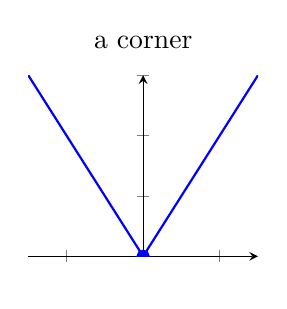
\begin{tikzpicture}
                        \begin{axis}[
                            title = a corner,
                            width = 4.5cm,
                            axis lines = middle,
                            yticklabels = {,,},
                            xticklabels = {,,},
                        ]
                        \addplot[
                            samples = 50,
                            thick,
                            color = blue,
                            domain = -3:0,
                        ]{-x};
                        \addplot[
                            samples = 50,
                            thick,
                            color = blue,
                            domain = 0:3,
                        ]{x};
                        \fill[blue,draw=blue,thick](axis cs:0,0)circle[radius=2pt];
                        \end{axis}
                    \end{tikzpicture}
                    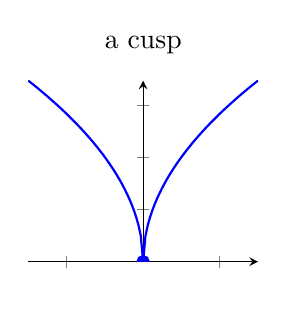
\begin{tikzpicture}
                        \begin{axis}[
                            title = a cusp,
                            width = 4.5cm,
                            axis lines = middle,
                            yticklabels = {,,},
                            xticklabels = {,,},
                        ]
                        \addplot[
                            samples = 50,
                            thick,
                            color = blue,
                            domain = -3:0,
                        ]{sqrt(-x)};
                        \addplot[
                            samples = 50,
                            thick,
                            color = blue,
                            domain = 0:3,
                        ]{sqrt(x)};
                        \fill[blue,draw=blue,thick](axis cs:0,0)circle[radius=2pt];
                        \end{axis}
                    \end{tikzpicture}
                    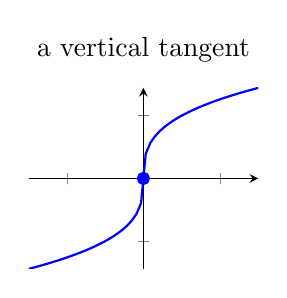
\begin{tikzpicture}
                        \begin{axis}[
                            title = a vertical tangent,
                            width = 4.5cm,
                            axis lines = middle,
                            yticklabels = {,,},
                            xticklabels = {,,},
                        ]
                        \addplot[
                            samples = 50,
                            thick,
                            color = blue,
                            domain = -3:3,
                        ]{x/abs(x)*abs(x)^(1/3)};
                        \fill[blue,draw=blue,thick](axis cs:0,0)circle[radius=2pt];
                        \end{axis}
                    \end{tikzpicture}
                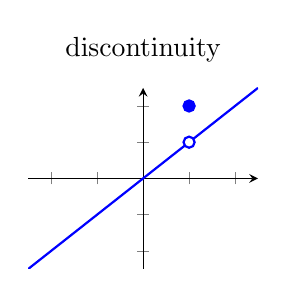
\begin{tikzpicture}
                        \begin{axis}[
                            title = discontinuity,
                            width = 4.5cm,
                            axis lines = middle,
                            yticklabels = {,,},
                            xticklabels = {,,},
                        ]
                        \addplot[
                            samples = 50,
                            thick,
                            color = blue,
                            domain = -5:5,
                        ]{x};
                        \fill[white,draw=blue,thick](axis cs:2,2)circle[radius=2pt];
                        \fill[blue,draw=blue,thick](axis cs:2,4)circle[radius=2pt];
                        \end{axis}
                    \end{tikzpicture}
        \end{itemize}
    \subsection{Differentiation Rules}
        \subsubsection{Constant Rule}
            for c = a constant
            \begin{gather*}
                c' = 0
            \end{gather*}
        \subsubsection{Constant Power Rule}
            \begin{gather*}
                (x^n)' = nx^{n-1}
            \end{gather*}
        \subsubsection{Variable Power Rule}
        Where c = a constant
            \begin{gather*}
                (a^{cx})' = ln(a^c) * \left(a^c\right)^x
            \end{gather*}
            Special case: 
            \begin{gather*}
                (e^{cx})' = ce^{cx}
            \end{gather*}
        \subsubsection{Sum Rule}
            \begin{gather*}
                (a(x) + z(x))' = a'(x) + z'(x)
            \end{gather*}
        \subsubsection{Quotient Rule}
            \begin{gather*}
                \left(\frac{a}{z}\right)' = \frac{\frac{da}{dx}*z-a*\frac{dz}{dx}}{z^2}
            \end{gather*}
        \subsubsection{Product Rule}
            \begin{gather*}
                (az)' = \frac{da}{dx}*z + a*\frac{dz}{dx}
            \end{gather*}
        \subsubsection{Trig Rules}
            \begin{multicols}{2}
                \begin{gather*}
                    \ddx\sin(x) = \cos(x)
                \end{gather*}
                \begin{gather*}
                    \ddx\tan(x) = \sec^2(x)
                \end{gather*}
                \begin{gather*}
                    \ddx\sec(x) = \sec(x)\tan(x)
                \end{gather*}
                \columnbreak
                \begin{gather*}
                   \ddx\cos(x) = -\sin(x)
                \end{gather*}
                \begin{gather*}
                    \ddx\cot(x) = -\csc^2(x)
                \end{gather*}
                \begin{gather*}
                    \ddx\csc(x) = -\csc(x)\cot(x)
                \end{gather*}
            \end{multicols}
        \subsubsection{Log Rule}
            \begin{gather*}
                (\log_au)' = \ddx\frac{\ln(u)}{\ln(a)} =  \frac{1}{u}*\frac{1}{\ln(a)}*\dd{u}{a}
            \end{gather*}
        \subsubsection{Natural Log Rule}
            \begin{gather*}
                \left(\ln(a)\right)' = \frac{1}{a}
            \end{gather*}
    \subsection{Physics}
        Displacement = change in position\\
        Velocity = \((\text{Displacement})'\)\\
        Acceleration = \((\text{Velocity})' = (\text{Displacement})''\)\\
        Speed = \(|\text{Velocity}| = \left|(\text{Displacement})'\right|\)
    \subsection{Marginal Cost/Revenue}
        If \(c(x)\) is the cost of producing x items, \(c'(x)\) is the  additional cost of producing \(x+1\) items, called the marginal cost. In other words, \(c(x) + c'(x)\) gives the total cost of producing \(x+1\) items. Marginal revenue is found the same way, using the function for revenue.
    \subsection{Chain Rule}
        Functions with other functions in them can be differentiated using the chain rule. For example,
        \begin{gather*}
            f(x) = (\sin(x))^3
        \end{gather*}
        Split into two functions, \(a\) and \(b\)
        \begin{gather*}
            a = b^3 \text{\tab} b = \sin(x)
        \end{gather*}
        \begin{gather*}
            f'(x) = a'(b) * b'(x) \text{\tab or \tab} \dd{f}{x} = \dd{a}{b}*\dd{b}{x}
        \end{gather*}
    \subsection{Implicit Differentiation}
        \begin{gather*}
            \text{if } a = b \text{ then } \dd{a}{x} = \dd{b}{x}
        \end{gather*}
    \subsection{Inverse Functions}
        \begin{gather*}
            \dd{x}{y} = \frac{1}{\dd{y}{x}}
        \end{gather*}
    \subsection{Rate of Change}
        if you have a function of time, any variable (for example \(x\)) in that function (for example \(f(x)\)) can be found by
        \begin{gather*}
            \dd{x}{f} * \dd{f}{t} = \dd{x}{t}
        \end{gather*}
\section{Differentials \& Linearization}
    \subsection{Linearization}
        if \(f\) is differentiable at \(x = a\), then the linearization of \(f\) is 
        \begin{gather*}
            L(x) = f(a) + f'(a)(x-a)
        \end{gather*}
    \subsection{Differentials}
        \(dy\) and \(dx\) are two variables with the property that when the ratio between then exists, the derivative exists.
        \begin{gather*}
            \Delta L = L(a+dx) - L(a)
        \end{gather*}
        \begin{gather*}
            \Delta L = f'(a)(dx) = dy
        \end{gather*}
        \subsubsection{Sensitivity to Change}
            Sensitivity to change problems deal with how accurately \(x\) must be measured in order to find the value of \(f(x)\) within some margin of error \(\frac{e}{100}\). This is illustrated by the equation 
            \begin{gather*}
                \frac{df}{f} \leq \frac{e}{100}
            \end{gather*}
            which should be solved for \(dx\)
\section{Extreme Values}
    Also known as maximums and minimums, maxima and minima, or extrema(s) 
    \subsection{Absolute Extrema}
        An absolute extremum is a point where the graph has the minimum or maximum y-value out of the entire domain.\\
        \\
        Not all functions are guaranteed to have an absolute minimum or maximum. The Extreme Value Theorem states that if a function \(f(x)\) is continuous on an interval \([a, b]\), then it is guaranteed to have some absolute minimum or maximum. This does not apply to a function \(f(x)\) that is continuous on an interval with one or both sides open.\\
        \\
        For example, given the continuous function \(f(x)\) and the domain \(D\) of \(f(x)\)
        \begin{gather*}
            f(x) \text{ has a maximum at } c \text{ if } f(x) \leq f(c) \text{ for all } x \text{ on } D
        \end{gather*}
        \centerline{and} 
        \begin{gather*}
            f(x) \text{ has a minimum at } c \text{ if } f(x) \geq f(c) \text{ for all } x \text{ on } D
        \end{gather*}
    \subsection{Local Extrema}
        Also known as Relative Extrema\\
        A local extremum is an extreme value relative to its surrounding points. they usually show up as peaks or troughs in the graph.\\
        To find the local extrema for a function \(f(x)\) that is continuous over the interval \(D\), one must find the critical points of \(f(x)\) that fall within \(D\), and the endpoints of \(f(x)\) within \(D\).
        \subsubsection{Critical Points}
            A function \(f(x)\) has a critical point at \(c\) when 
            \begin{gather*}
                f'(c) = 0
            \end{gather*}
            \centerline{or}
            \begin{gather*}
                f'(c) = undefined
            \end{gather*}
            given that \(f(c)\) exists\\
            Tip: factoring \(f'(x)\) or rewriting it as a fraction can make it easier to find critical points
\section{Mean Value Theorem}
    If a function \fx is both continuous on \([a, b]\) and differentiable on \((a, b)\), then there exists some value \(c\) within \((a, b)\) for which
    \begin{gather*}
        f(b)-f(a)=f'(c)(b-a) \text{\tab thus, } \frac{\Delta f}{\Delta x} = f'(c)
    \end{gather*}
    In other words, the average slope \(\frac{\Delta f}{\Delta x}\) of \(f(x)\) over the interval \([a, b]\) is the instantaneous (aka tangent) slope at some interior point.
    \subsection{Special case: Rolle's Theorem}
        if \(f(a) = f(b)\), then \(f'(c) = 0\) for some interior point \(c\)
    \subsection{Corollary 1}
    If \fx is continuous on \ciab, and \(f'(x)=0\) for all values of \(x\) within \((a, b)\), then \fx is constant on \ciab
    \subsection{Corollary 2}
    If \fx and \(g(x)\) are both continuous with the same derivative, then they differ by a constant.
\section{Monotone Functions}
    A function is considered monotone if it does not change direction (stays increasing, decreasing, or constant)
    \subsection{Increasing}
        An increasing function's outputs increase as its inputs increase
        \begin{gather*}
            \text{when } x_1 \leq x_2 \text{, } f(x_1) \leq f(x_2)
        \end{gather*}
    \subsection{Decreasing}
        A decreasing function's outputs decrease as its inputs increase
        \begin{gather*}
            \text{when } x_1 \leq x_2 \text{, } f(x_1) \geq f(x_2)
        \end{gather*}
    \subsection{First Derivative Test}
        The first derivative tells us whether the function is increasing or decreasing at a point.
        \begin{gather*}
            \text{If } f'> 0 \text{ on } (a, b) \text{, then } f \text{ is strictly increasing on } (a, b)
        \end{gather*}
        \begin{gather*}
            \text{If } f'< 0 \text{ on } (a, b) \text{, then } f \text{ is strictly decreasing on } (a, b)
        \end{gather*}
        \begin{gather*}
            \text{If } f'= 0 \text{ on } (a, b) \text{, then } f \text{ is constant on } (a, b)
        \end{gather*}
        This gives us the First Derivative Test: if \(x=c\) is a critical value, then it is a local extremum only if \(f'\) changes direction on opposite sides of \(c\)
        \subsubsection{Graphing the first Derivative Test}
            Mark the critical points on a number line and plot the signs for each interval.
\clearpage
\section{Concavity}
    \subsection{Concavity}
        Concavity shows how a graph curves, and is found with the second derivative
        \begin{gather*}
            \text{If } f''> 0 \text{ on } (a, b) \text{, then } f \text{ is concave up (a.k.a convex) on } (a, b)
        \end{gather*}
        \centerline{
            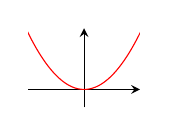
\begin{tikzpicture}
                \begin{axis}[
                    width = 3cm,
                    ticks = none,
                    axis lines = middle,
                    xlabel = \(\),
                    ylabel = \(\),
                    xmin = -2.5,
                    xmax = 2.5,
                    ymin = -.5,
                    ymax = 1.7,
                ]
                    \addplot[
                        samples = 100,
                        color = red,
                        domain = -3:3
                    ]{(x/2)^2};
                \end{axis}
            \end{tikzpicture}
        }
        \begin{gather*}
            \text{If } f''< 0 \text{ on } (a, b) \text{, then } f \text{ is concave down on } (a, b)
        \end{gather*}
        \centerline{
            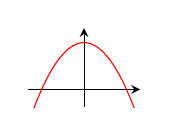
\begin{tikzpicture}
                \begin{axis}[
                    width = 3cm,
                    ticks = none,
                    axis lines = middle,
                    xlabel = \(\),
                    ylabel = \(\),
                    xmin = -3,
                    xmax = 3,
                    ymin = -.5,
                    ymax = 1.7,
                ]
                    \addplot[
                        samples = 100,
                        color = red,
                        domain = -3:3
                    ]{-(x/2)^2+1.3};
                \end{axis}
            \end{tikzpicture}
        }
        \begin{gather*}
            \text{If } f''= 0 \text{ on } (a, b) \text{, then } f \text{ is flat on } (a, b)
        \end{gather*}
        \centerline{
            \begin{tikzpicture}
                \begin{axis}[
                    width = 3cm,
                    ticks = none,
                    axis lines = middle,
                    xlabel = \(\),
                    ylabel = \(\),
                    xmin = -2.5,
                    xmax = 2.5,
                    ymin = -.5,
                    ymax = 1.7,
                ]
                    \addplot[
                        samples = 100,
                        color = red,
                        domain = -3:3
                    ]{1};
                \end{axis}
            \end{tikzpicture}
        }
        Points where concavity changes are called inflection points
        \subsubsection{Second Derivative Test}
            If \(x=c\) is a critical value, and \(f''(c) > 0\), then c is a local minimum.\\
            If \(x=c\) is a critical value, and \(f''(c) < 0\), then c is a local maximum. 
\section{Indeterminate Forms and L'Hôpital's rule}
    The indeterminate forms are 
    \begin{gather*}
        \frac{0}{0}\tab \frac{\infty}{\infty}\tab 0*\infty\tab 0^0\tab \infty^0\tab 1^\infty\tab \infty - \infty
    \end{gather*}
    
    \subsection{L'Hôpital's rule}
        L'Hôpital's rule states that
        \begin{gather*}
            \limxar\left(\frac{f(x)}{g(x)}\right)=\limxar\left(\frac{f'(x)}{g'(x)}\right)
        \end{gather*}
        if and only if
        \begin{gather*}
            \frac{f(x)}{g(x)} = \frac{0}{0} \text{ or } \frac{\infty}{\infty}
        \end{gather*}
        But exponential indeterminate forms (\(0^0, \infty^0, 1^\infty\)) can be manipulated to allow for the use of L'Hôpital's rule with the property
        \begin{gather*}
            \text{given } L=\limxa\left(\ln f(x)\right)
        \end{gather*}
        \begin{gather*}
            \limxa f(x) = \limxa \left(e^{\ln f(x)}\right) = e^L
        \end{gather*}
\section{Antiderivatives}
    The antiderivative, or indefinite integral, of a function is the function it is derived from. we use \(F(x)\) to denote the antiderivative of \fx. The most general antiderivative is 
    \begin{gather*}
        \int f(x)dx = F(x) + C
    \end{gather*}
    where \(C\) is a constant
\section{Finite Sums}
    \begin{gather*}
        \sum_{k=m}^{n} a_{k} = a_{m} + a_{m+1} + a_{m+2} + ... + a_n
    \end{gather*}
    \subsection{Algebra Rules for Finite Sums}
        \subsubsection{Constant Multiple Rule}
            \begin{gather*}
                \regsum Ca_k = C \regsum a_k
            \end{gather*}
        \subsubsection{Sum and Difference Rule}
            \begin{gather*}
                \regsum (a_k\pm b_k) = \regsum(a_k) \pm \regsum(b_k)
            \end{gather*}
        \subsubsection{Constant Value Rule}
            \begin{gather*}
                \regsum C = nC
            \end{gather*}
    \subsection{First \(n\) Numbers}
        \begin{gather*}
            \regsum k = \frac{n(n+1)}{2}
        \end{gather*}
        \subsubsection{First \(n\) Squares}
            \begin{gather*}
                \regsum k^2 = \frac{n(n+1)(2n+1)}{6}
            \end{gather*}
        \subsubsection{First \(n\) Cubes}
            \begin{gather*}
                \left(\frac{n(n+1)}{2}\right)^2
            \end{gather*}
\section{Definite Integrals}
    \subsection{Some rules}
        
    
\end{document}
